% =====================================================================
%  HELLO BUDDY — FULL USER MANUAL
%  Course   : Electronic Product Development (Sessional) — Lab
%  Standard : IEC/IEEE 82079-1 (Preparation of instructions for use),
%             ISO/IEC/IEEE 26514 (Information for users),
%             ANSI Z535.6 / ISO 3864 signal words (DANGER / WARNING /
%             CAUTION / NOTICE), ISO 7010 and IEC 60417 symbols,
%             IEC 62368-1 (Instructional safeguards), IEC 60529 (IP code).
% =====================================================================
\documentclass[11pt,a4paper,oneside]{report}
\usepackage[a4paper,margin=1in,headheight=14pt]{geometry}
\usepackage[T1]{fontenc}
\usepackage{helvet}
\usepackage{times}
\usepackage{amsmath,amssymb}
\usepackage{graphicx}
\usepackage{booktabs,array,longtable,tabularx,multirow}
\usepackage[table]{xcolor}
\usepackage{enumitem}
\usepackage{fancyhdr}
\usepackage{caption}
\usepackage{float}
\usepackage{lastpage}
\usepackage{makeidx}
\usepackage{tikz}
\usetikzlibrary{arrows.meta,shapes.geometric,positioning,calc,fit}
\usepackage[most]{tcolorbox}
\usepackage{titlesec}
\usepackage[colorlinks=true,linkcolor=NavyBlue,urlcolor=NavyBlue]{hyperref}
\setlength{\emergencystretch}{3em}
\makeindex

% ---------- COLOR PALETTE ----------
\definecolor{NavyBlue}{RGB}{31,56,100}
\definecolor{LightBlue}{RGB}{220,230,241}
\definecolor{WarnYellow}{RGB}{255,204,0}
\definecolor{BuddyGreen}{RGB}{34,197,94}
\definecolor{BuddyDark}{RGB}{20,20,22}
\definecolor{BuddyBone}{RGB}{245,245,240}
\definecolor{AlertRed}{RGB}{220,38,38}

\newcommand{\hdr}[1]{\cellcolor{LightBlue}\textbf{#1}}
\newcommand{\menu}[1]{\textsf{\textbf{#1}}}
\newcommand{\ui}[1]{\textsf{#1}}

% ---------- DOCUMENT FIELDS ----------
\newcommand{\ProductName}{Hello Buddy}
\newcommand{\ProductSubtitle}{Desktop Companion and Study Assistant Robot}
\newcommand{\ModelNo}{HB-S3-N16R8}
\newcommand{\InstituteName}{Kalinga Institute of Industrial Technology (KIIT)}
\newcommand{\DeptName}{School of Electronics Engineering}
\newcommand{\DocNo}{EPD/UM/2026/G09}
\newcommand{\DocRev}{1.0}
\newcommand{\FWVer}{3.0}
\newcommand{\SupportMail}{support.hellobuddy@kiit.ac.in}
\newcommand{\GroupNo}{Group 09}

% ---------- CHAPTER / HEADER STYLE ----------
\titleformat{\chapter}[display]{\bfseries\Huge\color{NavyBlue}\sffamily}{\filleft\Large\chaptertitlename\ \thechapter}{8pt}{\titlerule[1.2pt]\vspace{6pt}}
\titlespacing*{\chapter}{0pt}{-10pt}{24pt}
\titleformat{\section}{\Large\bfseries\color{NavyBlue}\sffamily}{\thesection}{0.6em}{}
\titleformat{\subsection}{\large\bfseries\color{NavyBlue}\sffamily}{\thesubsection}{0.6em}{}
\pagestyle{fancy}\fancyhf{}
\fancyhead[L]{\small\sffamily \ProductName\ User Manual}
\fancyhead[R]{\small\sffamily \DocNo\ Rev \DocRev}
\fancyfoot[C]{\small\sffamily Page \thepage\ of \pageref{LastPage}}
\renewcommand{\headrulewidth}{0.4pt}
\fancypagestyle{plain}{\fancyhf{}\fancyfoot[C]{\small\sffamily Page \thepage\ of \pageref{LastPage}}\renewcommand{\headrulewidth}{0pt}}

% ---------- SYMBOLS (ISO 7010 / IEC 60417) ----------
\newcommand{\warnsym}[1][0.55cm]{\begin{tikzpicture}[baseline=-0.1ex]
 \fill[WarnYellow,draw=black,line width=0.6pt,rounded corners=1pt] (0,0)--(#1,0)--(#1/2,#1*0.87)--cycle;
 \node[font=\bfseries\scriptsize] at (#1/2,#1*0.3) {!};\end{tikzpicture}}
\newcommand{\elecsym}[1][0.55cm]{\begin{tikzpicture}[baseline=-0.1ex]
 \fill[WarnYellow,draw=black,line width=0.6pt,rounded corners=1pt] (0,0)--(#1,0)--(#1/2,#1*0.87)--cycle;
 \fill[black] (#1*0.55,#1*0.68)--(#1*0.33,#1*0.34)--(#1*0.48,#1*0.34)--(#1*0.40,#1*0.12)--(#1*0.68,#1*0.45)--(#1*0.52,#1*0.45)--cycle;
 \end{tikzpicture}}
\newcommand{\hotsym}[1][0.55cm]{\begin{tikzpicture}[baseline=-0.1ex]
 \fill[WarnYellow,draw=black,line width=0.6pt,rounded corners=1pt] (0,0)--(#1,0)--(#1/2,#1*0.87)--cycle;
 \foreach \x in {0.34,0.5,0.66}{\draw[line width=0.5pt] (#1*\x,#1*0.15) .. controls (#1*\x+0.04,#1*0.3) and (#1*\x-0.04,#1*0.4) .. (#1*\x,#1*0.55);}
 \end{tikzpicture}}
\newcommand{\mandsym}[1][0.5cm]{\begin{tikzpicture}[baseline=-0.5ex]
 \fill[blue!70!black] (0,0) circle (#1/2);\node[white,font=\bfseries\small] at (0,0) {i};\end{tikzpicture}}
\newcommand{\weeesym}[1][0.5cm]{\begin{tikzpicture}[baseline=0pt,scale=#1/0.5cm]
 \draw[line width=0.6pt] (0.1,0.05) rectangle (0.4,0.32);\draw[line width=0.6pt] (0.05,0.32)--(0.45,0.32);
 \draw[line width=0.6pt] (0.2,0.32) arc(180:0:0.05);
 \draw[line width=0.8pt,red] (0,0)--(0.5,0.5);\draw[line width=0.8pt,red] (0,0.5)--(0.5,0);
 \fill (0,-0.12) rectangle (0.5,-0.04);\end{tikzpicture}}
\newcommand{\callout}[1]{\tikz[baseline=-0.6ex]\node[circle,draw=NavyBlue,fill=white,text=NavyBlue,inner sep=1.2pt,font=\bfseries\scriptsize]{#1};}
\newcommand{\led}[1]{\tikz[baseline=-0.5ex]\fill[#1,draw=black!60,line width=0.3pt] (0,0) circle (0.12cm);}

% ---------- SIGNAL-WORD BOXES (ANSI Z535.6 / ISO 3864) ----------
\newtcolorbox{danger}{enhanced,colback=red!6,colframe=red!75!black,boxrule=1pt,arc=2pt,left=5pt,right=5pt,top=4pt,bottom=4pt,
  title={\elecsym\ \ DANGER},fonttitle=\bfseries\sffamily,coltitle=white,colbacktitle=red!75!black}
\newtcolorbox{warning}{enhanced,colback=orange!8,colframe=orange!85!black,boxrule=1pt,arc=2pt,left=5pt,right=5pt,top=4pt,bottom=4pt,
  title={\warnsym\ \ WARNING},fonttitle=\bfseries\sffamily,coltitle=black,colbacktitle=orange!85!black}
\newtcolorbox{caution}{enhanced,colback=yellow!10,colframe=yellow!60!black,boxrule=1pt,arc=2pt,left=5pt,right=5pt,top=4pt,bottom=4pt,
  title={\warnsym\ \ CAUTION},fonttitle=\bfseries\sffamily,coltitle=black,colbacktitle=WarnYellow}
\newtcolorbox{notice}{enhanced,colback=blue!5,colframe=blue!60!black,boxrule=1pt,arc=2pt,left=5pt,right=5pt,top=4pt,bottom=4pt,
  title={NOTICE},fonttitle=\bfseries\sffamily,coltitle=white,colbacktitle=blue!60!black}
\newtcolorbox{tip}{enhanced,colback=green!5,colframe=green!45!black,boxrule=0.8pt,arc=2pt,left=5pt,right=5pt,top=3pt,bottom=3pt,
  title={\mandsym[0.38cm]\ \ TIP / NOTE},fonttitle=\bfseries\sffamily,coltitle=white,colbacktitle=green!45!black}

\begin{document}
\pagenumbering{roman}

% =====================================================================
%  TITLE PAGE
% =====================================================================
\begin{titlepage}
\sffamily\begin{center}
{\Large \textbf{\InstituteName}}\\[0.2cm]
{\large \DeptName}\\[0.15cm]
{\normalsize Bhubaneswar, Odisha, India}\\[1.0cm]

% Vector Graphic Representation of Hello Buddy Robot
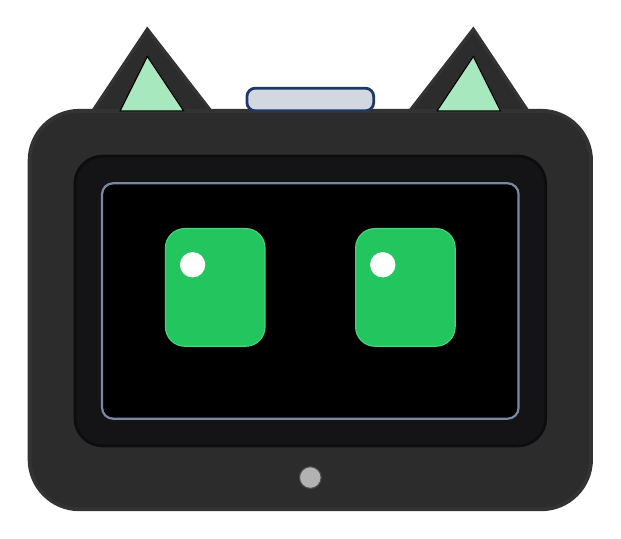
\begin{tikzpicture}[scale=1.15]
 % Robot Outer Head
 \draw[fill=BuddyDark!90,draw=black!80,line width=1.4pt,rounded corners=18pt] (0,0) rectangle (6.2,4.4);
 % Inner Face Screen Bezel
 \draw[fill=BuddyDark,draw=black!95,line width=1pt,rounded corners=10pt] (0.5,0.7) rectangle (5.7,3.9);
 % OLED Active Display Area (SH1106 128x64)
 \draw[fill=black,draw=NavyBlue!60,line width=0.8pt,rounded corners=4pt] (0.8,1.0) rectangle (5.4,3.6);
 % Left Eye (Happy/Neutral rounded rectangle eye)
 \draw[fill=BuddyGreen,draw=BuddyGreen!80,rounded corners=7pt] (1.5,1.8) rectangle (2.6,3.1);
 % Right Eye
 \draw[fill=BuddyGreen,draw=BuddyGreen!80,rounded corners=7pt] (3.6,1.8) rectangle (4.7,3.1);
 % Animated Eye Highlights
 \fill[white] (1.8,2.7) circle (0.14);
 \fill[white] (3.9,2.7) circle (0.14);
 % Chin Microphone Hole
 \fill[black!30,draw=black!70] (3.1,0.35) circle (0.12);
 % Top Capacitive Touch Pad Indicator
 \draw[fill=NavyBlue!20,draw=NavyBlue,line width=1pt,rounded corners=3pt] (2.4,4.4) rectangle (3.8,4.65);
 % Left and Right Cat Ears / Antennae
 \draw[fill=BuddyDark!90,draw=black!80,line width=1.2pt] (0.7,4.4)--(1.3,5.3)--(2.0,4.4)--cycle;
 \draw[fill=BuddyDark!90,draw=black!80,line width=1.2pt] (4.2,4.4)--(4.9,5.3)--(5.5,4.4)--cycle;
 \draw[fill=BuddyGreen!40] (1.0,4.4)--(1.3,5.0)--(1.7,4.4)--cycle;
 \draw[fill=BuddyGreen!40] (4.5,4.4)--(4.9,5.0)--(5.2,4.4)--cycle;
\end{tikzpicture}\\[0.8cm]

{\Huge\bfseries\color{NavyBlue} \ProductName}\\[0.25cm]
{\large\textbf{\ProductSubtitle}}\\[0.2cm]
{\normalsize Hardware Model: \textbf{\ModelNo} \quad\textbullet\quad Firmware: \textbf{v\FWVer}}\\[0.6cm]

\rule{0.75\linewidth}{1.0pt}\\[0.4cm]
{\Huge\bfseries USER MANUAL}\\[0.3cm]
{\large Installation \textbullet\ Voice \& App Operation \textbullet\ Maintenance \textbullet\ Troubleshooting}\\[0.4cm]
\rule{0.75\linewidth}{1.0pt}
\vfill

\renewcommand{\arraystretch}{1.25}
\begin{tabular}{rl}
\textbf{Document Number:} & \DocNo \\
\textbf{Course Code / Name:} & Electronic Product Development (Sessional) --- Lab \\
\textbf{Design Team:} & Group 09 (Ziaur Rahaman, Aryan Raj, Ayush Dutta, Shamil Minhaj) \\
\textbf{Supervising Faculty:} & Dr.\ Deepak Kumar Rout \\
\textbf{Document Revision:} & \DocRev \\
\textbf{Date of Issue:} & November 2026 \\
\end{tabular}\\[0.6cm]

{\small\warnsym\ \ \textbf{Important: Read this manual, especially Chapter~\ref{ch:safety}, before operating the product. Keep it for reference.}}
\end{center}
\end{titlepage}

% =====================================================================
%  NOTICES, REVISION HISTORY
% =====================================================================
\chapter*{Notices and Document Information}
\addcontentsline{toc}{chapter}{Notices and Document Information}

\section*{Copyright and Legal Disclaimer}
\copyright\ 2026 \InstituteName, \DeptName. All rights reserved. No part of this user manual may be reproduced, stored in a retrieval system, or transmitted in any form or by any means, electronic, mechanical, photocopying, recording, or otherwise, without prior written permission from the institution.

The information in this manual has been verified against physical hardware and firmware version \FWVer. Specifications are subject to change without notice in line with ongoing engineering improvements. All product names, logos, and brands (including Espressif\textsuperscript{\textregistered}, Groq\textsuperscript{\textregistered}, Firebase\textsuperscript{\textregistered}, Flutter\textsuperscript{\textregistered}, and Android\textsuperscript{\texttrademark}) are property of their respective owners.

\begin{notice}
\textbf{Educational Prototype Classification:} \ProductName\ is an interactive desktop companion developed as a comprehensive engineering capstone project under the \emph{Electronic Product Development (Sessional)} curriculum. This device is an engineered working prototype and has not undergone commercial third-party CE/FCC laboratory testing. It is intended for indoor desktop use under specified operating limits.
\end{notice}

\section*{Document Revision History}
\begin{table}[H]\centering\small
\caption{Document revision history}
\begin{tabular}{|c|c|p{0.48\linewidth}|c|}\hline
\hdr{Rev.} & \hdr{Date} & \hdr{Description of Changes} & \hdr{Firmware}\\ \hline
0.1 & 18-09-2026 & Initial draft generated following Product Design Report (PDR) & v1.0 \\ \hline
0.5 & 25-10-2026 & Updated I2S audio architecture (INMP441 + MAX98357A) & v2.0 \\ \hline
1.0 & 03-11-2026 & Final release with unified Groq Whisper STT, edge touch filter, and Flutter app actions & v\FWVer \\ \hline
\end{tabular}
\end{table}

\section*{Related Project Documentation}
\begin{table}[H]\centering\small
\caption{Cross-referenced design documentation}
\begin{tabular}{|l|l|p{0.42\linewidth}|}\hline
\hdr{Document Type} & \hdr{Document Number} & \hdr{Description}\\ \hline
Requirements Specification (RSD) & EPD/RSD/2026/G09 & Stakeholder and functional requirements \\ \hline
Product Design Report (PDR) & G09\_HelloBuddy\_PDR\_v1 & Mechanical, circuit, and firmware design \\ \hline
Flutter Companion App Spec & EPD/FAS/2026/G09 & Mobile architecture, UI flow, and Firebase \\ \hline
Product Test Report (PTR) & EPD/PTR/2026/G09 & Verification testing and validation records \\ \hline
\end{tabular}
\end{table}

\clearpage
\tableofcontents
\clearpage
\listoffigures
\clearpage
\listoftables
\clearpage
\pagenumbering{arabic}

% =====================================================================
%  ABOUT THIS MANUAL
% =====================================================================
\chapter*{About This Manual}
\addcontentsline{toc}{chapter}{About This Manual}

\section*{Intended Audience}
This manual is written for students, researchers, knowledge workers, and hobbyists who operate \textbf{\ProductName}. No prior programming or advanced electronics knowledge is required for everyday operation. Sections marked with \emph{Technician Only} contain hardware pinout mappings and low-level diagnostic routines intended for qualified personnel.

\section*{Manual Organization}
\begin{table}[H]\centering\small
\caption{Manual structural overview}
\begin{tabularx}{\linewidth}{|l|X|}\hline
\hdr{Chapter} & \hdr{Contents and Practical Purpose}\\ \hline
1~Safety Information & Personal safety precautions, electrical limits, and hazard warnings\\ \hline
2~Product Overview & Unboxing checklist, vector hardware layout, block diagram, and specifications\\ \hline
3~Installation and Setup & Desktop placement, USB-C power connection, Wi-Fi setup, and pairing\\ \hline
4~Operation & Expressions, voice command workflow, Pomodoro mode, and app control\\ \hline
5~Maintenance & Cleaning guidelines, firmware updating, storage, and replacement parts\\ \hline
6~Troubleshooting & Diagnostic decision tree, symptom resolution table, and error codes\\ \hline
7~Disposal and Environment & Environmental compliance, e-waste guidelines, and recycling routes\\ \hline
8~Warranty and Compliance & Warranty coverage, developer contact information, and compliance claims\\ \hline
Appendices & Quick reference cheat sheet, pin assignments, REST APIs, and glossary\\ \hline
\end{tabularx}
\end{table}

\section*{Safety and Signal Word Conventions (ANSI Z535.6)}
\begin{table}[H]\centering\small
\caption{Standard hazard alert classification}
\begin{tabularx}{\linewidth}{|c|l|X|}\hline
\hdr{Icon} & \hdr{Signal Word} & \hdr{Definition (Severity Level)}\\ \hline
\elecsym & \textbf{DANGER} & Indicates a hazardous situation that, if not avoided, \textbf{will} result in death or serious electrical injury.\\ \hline
\warnsym & \textbf{WARNING} & Indicates a hazardous situation that, if not avoided, \textbf{could} result in serious injury or equipment destruction.\\ \hline
\warnsym & \textbf{CAUTION} & Indicates a hazardous situation that, if not avoided, could result in minor or moderate injury.\\ \hline
--- & \textbf{NOTICE} & Addresses practices not related to personal injury (e.g., memory corruption or ESD damage).\\ \hline
\mandsym & \textbf{TIP / NOTE} & Highlights helpful operational advice, productivity tips, or recommended shortcuts.\\ \hline
\ui{[Text]} & Sans-serif bold & Identifies physical/virtual buttons, mobile app tabs, and displayed text.\\ \hline
\callout{1} & Numbered circle & Refers to a numbered mechanical or electrical part in illustrations.\\ \hline
\end{tabularx}
\end{table}

% =====================================================================
%  CHAPTER 1: SAFETY INFORMATION
% =====================================================================
\chapter{Safety Information}\label{ch:safety}
\index{safety}

\section{Intended Use}
\ProductName\ is an indoor, stationary desktop companion and study assistant robot designed to assist students and professionals with Pomodoro focus timing, task organization, natural language question answering, local weather updates, and background music playback. 

Operate \ProductName\ strictly in accordance with the ambient conditions, electrical specifications, and instructions detailed throughout this manual.

\begin{warning}
\textbf{Foreseeable Misuse Prohibition:}
\begin{itemize}[leftmargin=*]
\item Do \textbf{not} use \ProductName\ in medical, life-support, clinical patient-monitoring, or mission-critical automation systems.
\item Do \textbf{not} expose the device to rain, splashing liquids, high-humidity bathrooms, or outdoor weather.
\item Do \textbf{not} power the robot from unregulated, non-isolated, or automotive power supplies exceeding 5.25\,V\,DC.
\item Misuse voids all warranty claims and releases the design team from liability.
\end{itemize}
\end{warning}

\section{General Safety Instructions}
\begin{itemize}[leftmargin=*]
\item Inspect the enclosure, USB-C power cable, and power adapter before each use.
\item Position the device on a flat, dry, level desk surface away from desk edges to avoid accidental drops.
\item Ensure adequate ambient airflow around the back acoustic port and bottom vents.
\item Disconnect the power cable immediately if the robot emits smoke, unusual odors, or excessive heat.
\item Keep small hardware accessories away from infants and pets.
\end{itemize}

\section{Electrical Safety}\index{electrical safety}
\begin{danger}
\textbf{Electric Shock and Short-Circuit Hazards:}
\begin{itemize}[leftmargin=*]
\item Never insert metal wires, needles, or foreign objects into the microphone aperture, speaker grille, or OLED display seams.
\item Do not open the enclosure while the USB-C power cable is connected. Internal components operate on low-voltage DC (3.3\,V and 5.0\,V), but connected mains adapters carry lethal 100--240\,V\,AC line voltages.
\item Do not touch the power adapter or USB plug with wet or damp hands.
\end{itemize}
\end{danger}

\section{Acoustic and Thermal Safeguards}
\begin{caution}
\textbf{Acoustic Output Protection:} The MAX98357A internal Class-D amplifier drives an onboard 3\,W speaker capable of generating transient sound levels up to 82\,dB(A) at 0.5\,m. Avoid placing your ear directly against the rear speaker grille during high-volume chimes or voice playback.
\end{caution}

\begin{notice}
\textbf{Thermal and Electrostatic Precautions:}
\begin{itemize}[leftmargin=*]
\item The ESP32-S3 dual-core processor operates at 240\,MHz with active Wi-Fi and I2S DMA. Internal temperatures may rise 15--20\,\textdegree C above ambient during sustained operations. Never cover the robot with paper or fabric.
\item The capacitive touch sensor is sensitive to electrostatic discharge (ESD). Discharge personal static on an grounded metal surface before touching the robot in dry winter environments.
\end{itemize}
\end{notice}

\section{Product Safety Symbols}
\begin{table}[H]\centering\small
\caption{Safety and compliance labeling}
\begin{tabularx}{\linewidth}{|c|X|l|}\hline
\hdr{Symbol} & \hdr{Meaning / Instruction} & \hdr{Normative Reference}\\ \hline
\mandsym & Mandatory action: Read user instructions prior to operating & ISO 7010-M002\\ \hline
\elecsym & Electrical hazard: Risk of electric shock from damaged supply & ISO 7010-W012\\ \hline
\weeesym & Separate collection: Do not discard with unsorted municipal waste & WEEE Directive 2012/19/EU\\ \hline
--- & Direct current (DC) electrical input (5\,V\,DC $\pm$5\%) & IEC 60417-5031\\ \hline
--- & For indoor office and household use only & IEC 60417-5957\\ \hline
\end{tabularx}
\end{table}

% =====================================================================
%  CHAPTER 2: PRODUCT OVERVIEW
% =====================================================================
\chapter{Product Overview}\label{ch:overview}
\index{product overview}

\section{System Description and Key Features}
\ProductName\ (Model \textbf{\ModelNo}) integrates embedded edge intelligence, digital audio processing, and cloud AI services to provide an engaging desktop presence. 

\textbf{Core Capabilities:}
\begin{itemize}[leftmargin=*]
\item \textbf{High-Speed Edge STT Pipeline:} Uses dual-slot I2S DMA on an INMP441 MEMS microphone with on-chip high-pass DC filtering, uploading to Groq Whisper Large-v3-Turbo for speech recognition in under 400\,ms, with automatic fallback to Wit.ai.
\item \textbf{Generative Intelligence:} Cloud LLM processing (Qwen 3.8 / Llama 3.3 via Groq LPU) capable of parsing voice commands into structured actions (alarms, tasks, reminders).
\item \textbf{Expressive Visual Display:} 1.3'' SH1106 128$\times$64 OLED display rendering 8 distinct animated emotional states (Neutral, Happy, Listening, Thinking, Speaking, Alert, Sleepy, Sceptical).
\item \textbf{Natural Voice Synthesis:} Groq Orpheus neural WAV TTS output supported by native VoiceRSS fallback streamed to an I2S MAX98357A amplifier.
\item \textbf{Bidirectional Companion App Sync:} Real-time telemetry, remote expression control, music streaming via Audius API, and phone alarm synchronization via Google Firebase Realtime Database.
\end{itemize}

\section{Package Contents (Unboxing Checklist)}\label{sec:box}
\begin{table}[H]\centering\small
\caption{Package contents inspection list}
\begin{tabularx}{\linewidth}{|c|X|c|c|}\hline
\hdr{No.} & \hdr{Item Description} & \hdr{Qty} & \hdr{Verified}\\ \hline
1 & \ProductName\ Desktop Companion Robot (Model \ModelNo) & 1 & $\square$\\ \hline
2 & High-speed USB Type-C braided power and data cable (1.2\,m) & 1 & $\square$\\ \hline
3 & Regulated 5\,V\,DC / 2.0\,A USB wall adapter (Type A/C) & 1 & $\square$\\ \hline
4 & Quick Start Guide (one-page foldout with pairing QR code) & 1 & $\square$\\ \hline
5 & Quality inspection and academic warranty card & 1 & $\square$\\ \hline
\end{tabularx}
\end{table}
If any component is missing or damaged upon delivery, immediately notify \SupportMail\ before applying power.

\section{Hardware Layout and Controls}\label{sec:parts}
\index{hardware layout}\index{controls}

\begin{figure}[H]\centering
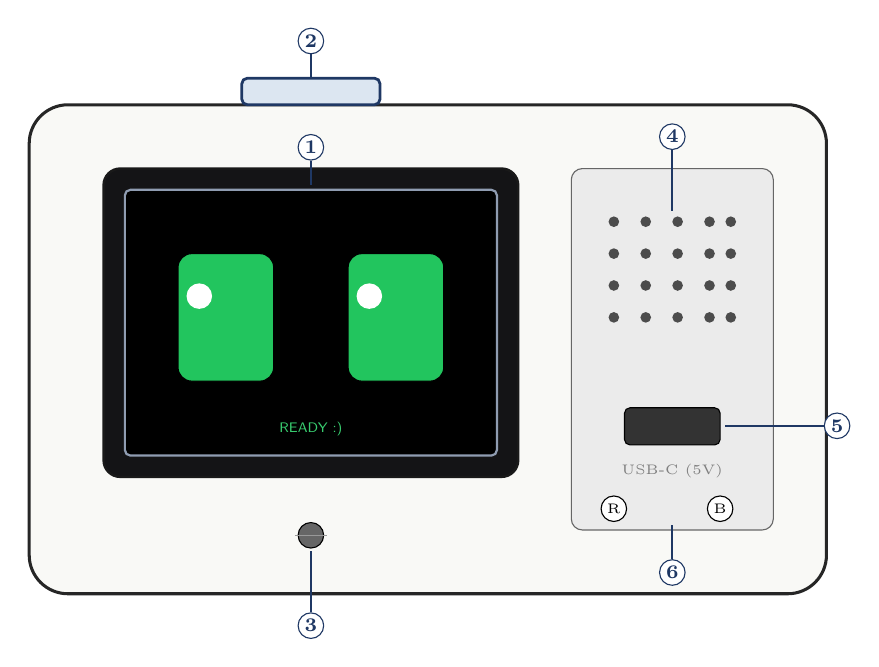
\begin{tikzpicture}[x=1.35cm,y=1.35cm,font=\footnotesize]
 % Outer Enclosure Body
 \draw[fill=BuddyBone!60,draw=black!85,line width=1.1pt,rounded corners=14pt] (0,0) rectangle (7.5,4.6);
 % OLED Bezel
 \draw[fill=BuddyDark,draw=black!90,line width=0.9pt,rounded corners=6pt] (0.7,1.1) rectangle (4.6,4.0);
 % Screen
 \draw[fill=black,draw=NavyBlue!50,line width=0.8pt,rounded corners=2pt] (0.9,1.3) rectangle (4.4,3.8);
 % Robot Eyes
 \draw[fill=BuddyGreen,rounded corners=5pt] (1.4,2.0) rectangle (2.3,3.2);
 \draw[fill=BuddyGreen,rounded corners=5pt] (3.0,2.0) rectangle (3.9,3.2);
 \fill[white] (1.6,2.8) circle (0.12);
 \fill[white] (3.2,2.8) circle (0.12);
 % Status Label on Screen
 \node[text=BuddyGreen!90,font=\sffamily\tiny] at (2.65,1.55) {READY :)};

 % Touch Sensor Crown Area
 \draw[fill=LightBlue,draw=NavyBlue,line width=1pt,rounded corners=2pt] (2.0,4.6) rectangle (3.3,4.85);

 % Microphone Aperture
 \draw[fill=black!60] (2.65,0.55) circle (0.12);
 \draw[black!40,line width=0.5pt] (2.5,0.55)--(2.8,0.55);

 % Right Side Control Panel (Speaker & Ports)
 \draw[fill=black!8,draw=black!60,rounded corners=4pt] (5.1,0.6) rectangle (7.0,4.0);
 % Speaker Grille
 \foreach \y in {2.6, 2.9, 3.2, 3.5} {
   \foreach \x in {5.5, 5.8, 6.1, 6.4, 6.6} {
     \fill[black!70] (\x,\y) circle (0.05);
   }
 }
 % USB-C Port
 \draw[fill=black!80,rounded corners=2pt] (5.6,1.4) rectangle (6.5,1.75);
 \node[font=\tiny,text=black!50] at (6.05,1.15) {USB-C (5V)};

 % Hardware EN / BOOT Buttons
 \draw[fill=white,draw=black] (5.5,0.8) circle (0.12);\node[font=\tiny] at (5.5,0.8) {R};
 \draw[fill=white,draw=black] (6.5,0.8) circle (0.12);\node[font=\tiny] at (6.5,0.8) {B};

 % Callout Indicators
 \node[circle,draw=NavyBlue,fill=white,inner sep=1pt,text=NavyBlue,font=\bfseries\scriptsize] (c1) at (2.65,4.2) {1};
 \draw[NavyBlue,line width=0.7pt] (c1)--(2.65,3.85);

 \node[circle,draw=NavyBlue,fill=white,inner sep=1pt,text=NavyBlue,font=\bfseries\scriptsize] (c2) at (2.65,5.2) {2};
 \draw[NavyBlue,line width=0.7pt] (c2)--(2.65,4.85);

 \node[circle,draw=NavyBlue,fill=white,inner sep=1pt,text=NavyBlue,font=\bfseries\scriptsize] (c3) at (2.65,-0.3) {3};
 \draw[NavyBlue,line width=0.7pt] (c3)--(2.65,0.4);

 \node[circle,draw=NavyBlue,fill=white,inner sep=1pt,text=NavyBlue,font=\bfseries\scriptsize] (c4) at (6.05,4.3) {4};
 \draw[NavyBlue,line width=0.7pt] (c4)--(6.05,3.6);

 \node[circle,draw=NavyBlue,fill=white,inner sep=1pt,text=NavyBlue,font=\bfseries\scriptsize] (c5) at (7.6,1.58) {5};
 \draw[NavyBlue,line width=0.7pt] (c5)--(6.55,1.58);

 \node[circle,draw=NavyBlue,fill=white,inner sep=1pt,text=NavyBlue,font=\bfseries\scriptsize] (c6) at (6.05,0.2) {6};
 \draw[NavyBlue,line width=0.7pt] (c6)--(6.05,0.65);
\end{tikzpicture}
\caption{\ProductName\ front and side interface callouts}\label{fig:parts}
\end{figure}

\begin{table}[H]\centering\small
\caption{Interface callout description table (see Figure~\ref{fig:parts})}
\begin{tabularx}{\linewidth}{|c|l|X|}\hline
\hdr{No.} & \hdr{Component / Port} & \hdr{Functional Purpose}\\ \hline
\callout{1} & SH1106 OLED Display & 128$\times$64 4-wire SPI screen displaying real-time animated eyes, status text, and IP\\ \hline
\callout{2} & TTP223 Capacitive Touch Crown & Touch-sensitive head region; single touch triggers listening mode; 80\,ms debounce\\ \hline
\callout{3} & INMP441 Acoustic Port & Precision acoustic aperture exposing the 24-bit MEMS microphone capsule\\ \hline
\callout{4} & Speaker Acoustic Grille & Tuned sound chamber output for the 3\,W 4\,$\Omega$ high-clarity speaker driver\\ \hline
\callout{5} & USB-C Input / Flash Port & Main 5\,V\,DC / 2\,A power input and CP2102/CH343 serial flashing interface\\ \hline
\callout{6} & Hardware Reset (EN) \& Boot & Recessed momentary buttons for system reboot and flashing bootloader entry\\ \hline
\end{tabularx}
\end{table}

\begin{tip}
\textbf{Optional Hardware Visuals:} If you have actual studio photographs or CAD rendering exports of the Hello Buddy chassis, place them inside a \texttt{figures/} subfolder (e.g., \texttt{figures/robot\_front.png}) and replace the TikZ diagram in Figure~\ref{fig:parts} with \texttt{\textbackslash includegraphics[width=0.85\textbackslash linewidth]\{figures/robot\_front.png\}}.
\end{tip}

\section{Hardware Architecture and Bus Topology}\label{sec:hw_arch}
Figure~\ref{fig:hw_architecture} details the comprehensive physical hardware architecture, electrical power distribution, and multi-bus topology of \ProductName. The architecture isolates high-speed digital buses, analog audio paths, and wireless radio interfaces to eliminate clock crosstalk and ensure pristine audio capture.

\begin{figure}[H]\centering
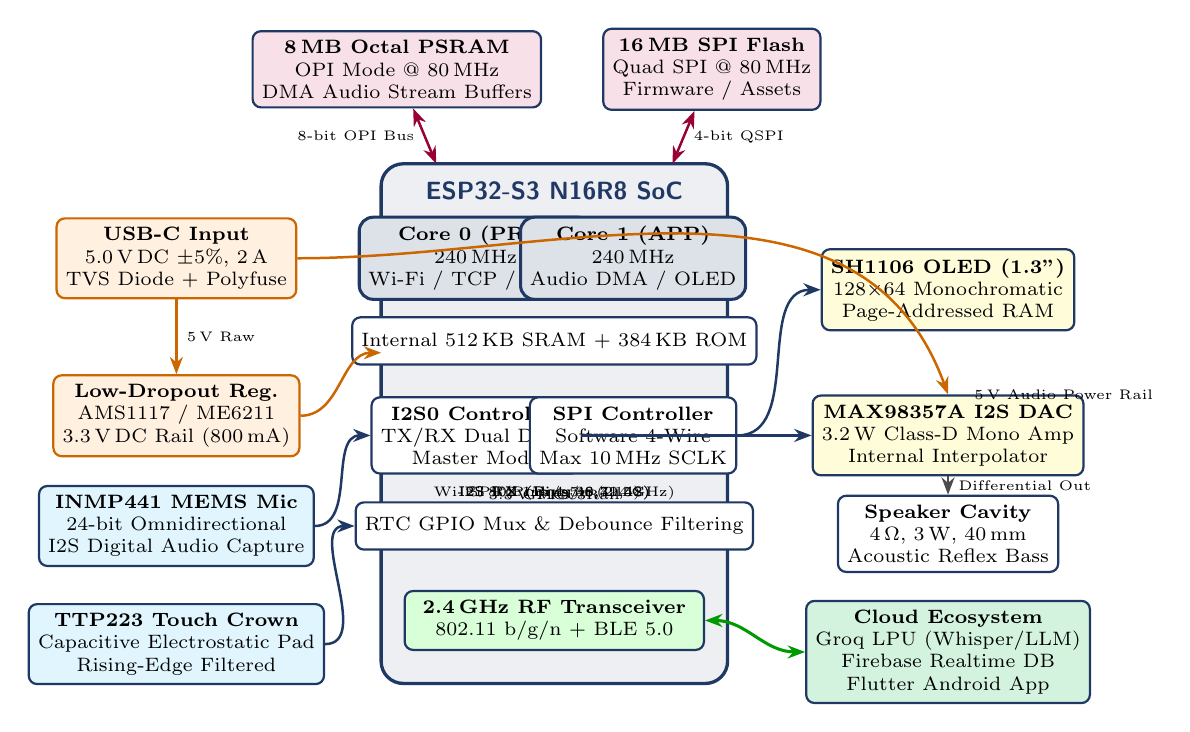
\begin{tikzpicture}[font=\scriptsize,
 blk/.style={draw=NavyBlue,fill=LightBlue!40,rounded corners=3pt,align=center,line width=0.8pt},
 mcu/.style={draw=NavyBlue,fill=NavyBlue!15,rounded corners=5pt,align=center,line width=1.1pt},
 pwr/.style={draw=orange!80!black,fill=orange!12,rounded corners=3pt,align=center,line width=0.8pt},
 bus/.style={-{Stealth[length=2.2mm]},line width=0.9pt},
 dbus/.style={{Stealth[length=2.2mm]}-{Stealth[length=2.2mm]},line width=0.9pt}]

 % Power Subsystem (Left)
 \node[pwr,minimum width=2.4cm,minimum height=1.0cm] (usbin) at (-4.8,3.2) {\textbf{USB-C Input}\\5.0\,V\,DC $\pm$5\%, 2\,A\\TVS Diode + Polyfuse};
 \node[pwr,minimum width=2.4cm,minimum height=0.9cm] (ldo) at (-4.8,1.2) {\textbf{Low-Dropout Reg.}\\AMS1117 / ME6211\\3.3\,V\,DC Rail (800\,mA)};
 \draw[bus,draw=orange!80!black] (usbin)--(ldo) node[midway,right,font=\tiny] {5\,V Raw};

 % Central ESP32-S3 SoC (Core of System)
 \draw[draw=NavyBlue,fill=NavyBlue!8,rounded corners=8pt,line width=1.2pt] (-2.2,-2.2) rectangle (2.2,4.4);
 \node[NavyBlue,font=\sffamily\bfseries\small] at (0,4.05) {ESP32-S3 N16R8 SoC};

 % Internal SoC Core Blocks
 \node[mcu,minimum width=1.8cm,minimum height=0.7cm] (c0) at (-1.0,3.2) {\textbf{Core 0 (PRO)}\\240\,MHz\\Wi-Fi / TCP / RTOS};
 \node[mcu,minimum width=1.8cm,minimum height=0.7cm] (c1) at (1.0,3.2) {\textbf{Core 1 (APP)}\\240\,MHz\\Audio DMA / OLED};
 \node[blk,minimum width=3.8cm,minimum height=0.6cm,fill=white] (sram) at (0,2.15) {Internal 512\,KB SRAM + 384\,KB ROM};
 \node[blk,minimum width=1.8cm,minimum height=0.7cm,fill=white] (i2s) at (-1.0,0.95) {\textbf{I2S0 Controller}\\TX/RX Dual DMA\\Master Mode};
 \node[blk,minimum width=1.8cm,minimum height=0.7cm,fill=white] (spi) at (1.0,0.95) {\textbf{SPI Controller}\\Software 4-Wire\\Max 10\,MHz SCLK};
 \node[blk,minimum width=3.8cm,minimum height=0.6cm,fill=white] (gpio_ctrl) at (0,-0.2) {RTC GPIO Mux \& Debounce Filtering};
 \node[blk,minimum width=3.8cm,minimum height=0.7cm,fill=green!15] (rf) at (0,-1.4) {\textbf{2.4\,GHz RF Transceiver}\\802.11 b/g/n + BLE 5.0};

 % Top Memory Subsystem
 \node[blk,minimum width=2.3cm,minimum height=0.9cm,fill=purple!12] (psram) at (-2.0,5.6) {\textbf{8\,MB Octal PSRAM}\\OPI Mode @ 80\,MHz\\DMA Audio Stream Buffers};
 \node[blk,minimum width=2.3cm,minimum height=0.9cm,fill=purple!12] (flash) at (2.0,5.6) {\textbf{16\,MB SPI Flash}\\Quad SPI @ 80\,MHz\\Firmware / Assets};
 \draw[dbus,draw=purple!80!black] (psram)--(-1.5,4.4) node[midway,left,font=\tiny] {8-bit OPI Bus};
 \draw[dbus,draw=purple!80!black] (flash)--(1.5,4.4) node[midway,right,font=\tiny] {4-bit QSPI};

 % External Peripherals - Input (Bottom Left)
 \node[blk,minimum width=2.5cm,minimum height=0.95cm,fill=cyan!12] (mic) at (-4.8,-0.2) {\textbf{INMP441 MEMS Mic}\\24-bit Omnidirectional\\I2S Digital Audio Capture};
 \node[blk,minimum width=2.5cm,minimum height=0.85cm,fill=cyan!12] (touch) at (-4.8,-1.7) {\textbf{TTP223 Touch Crown}\\Capacitive Electrostatic Pad\\Rising-Edge Filtered};

 % External Peripherals - Output (Bottom Right)
 \node[blk,minimum width=2.6cm,minimum height=0.95cm,fill=yellow!15] (amp) at (5.0,0.95) {\textbf{MAX98357A I2S DAC}\\3.2\,W Class-D Mono Amp\\Internal Interpolator};
 \node[blk,minimum width=2.4cm,minimum height=0.7cm,fill=white] (spk) at (5.0,-0.3) {\textbf{Speaker Cavity}\\4\,$\Omega$, 3\,W, 40\,mm\\Acoustic Reflex Bass};
 \node[blk,minimum width=2.6cm,minimum height=0.95cm,fill=yellow!15] (oled) at (5.0,2.8) {\textbf{SH1106 OLED (1.3")}\\128$\times$64 Monochromatic\\Page-Addressed RAM};

 % External Cloud / Mobile (Right Side)
 \node[blk,minimum width=2.8cm,minimum height=1.0cm,fill=BuddyGreen!20] (cloud) at (5.0,-1.8) {\textbf{Cloud Ecosystem}\\Groq LPU (Whisper/LLM)\\Firebase Realtime DB\\Flutter Android App};

 % Power Connections
 \draw[bus,draw=orange!80!black] (usbin.east) to[out=0,in=110] (amp.north) node[above=0.4cm,right=0.2cm,font=\tiny] {5\,V Audio Power Rail};
 \draw[bus,draw=orange!80!black] (ldo.east) to[out=0,in=180] (-2.2,2.0) node[midway,above,font=\tiny] {3.3\,V MCU Rail};

 % Audio & Signal Interconnects
 \draw[bus,draw=NavyBlue] (mic.east) to[out=0,in=180] (i2s.west) node[midway,above,font=\tiny] {I2S RX (Pins 40,41,42)};
 \draw[bus,draw=NavyBlue] (touch.east) to[out=0,in=180] (gpio_ctrl.west) node[midway,above,font=\tiny] {GPIO 3};
 \draw[bus,draw=NavyBlue] (i2s.east) to[out=0,in=180] (amp.west) node[midway,above,font=\tiny] {I2S TX (Pins 38,39,48)};
 \draw[bus,draw=black!70] (amp)--(spk) node[midway,right,font=\tiny] {Differential Out};
 \draw[bus,draw=NavyBlue] (spi.east) to[out=0,in=180] (oled.west) node[midway,above,font=\tiny] {SPI (Pins 4,5,6,7,15)};
 \draw[dbus,draw=green!60!black,line width=1.1pt] (rf.east) to[out=0,in=180] (cloud.west) node[midway,above,font=\tiny] {Wi-Fi 802.11b/g/n (2.4\,GHz)};
\end{tikzpicture}
\caption{Hello Buddy comprehensive hardware architecture and multi-bus topology}\label{fig:hw_architecture}
\end{figure}

\begin{table}[H]\centering\small
\caption{System bus architecture and hardware interconnect mapping}
\begin{tabularx}{\linewidth}{|l|l|l|l|X|}\hline
\hdr{Subsystem Bus} & \hdr{Protocol / Mode} & \hdr{Clock / Baud} & \hdr{Pin Allocations} & \hdr{Functional Purpose}\\ \hline
OPI PSRAM & Octal SPI (8-bit) & 80\,MHz SDR & Dedicated Internal & 8\,MB buffer for 1\,MB TTS streams and 96\,KB WAVs\\ \hline
QSPI Flash & Quad SPI (4-bit) & 80\,MHz & Dedicated Internal & 16\,MB non-volatile storage for bootloader and firmware\\ \hline
I2S0 Capture & Philips I2S (24-bit) & 1.024\,MHz BCLK & SCK=42, WS=41, SD=40 & 16\,kHz 16-bit digital audio streaming from INMP441\\ \hline
I2S0 Playback & Philips I2S (16-bit) & Dynamic (24/16\,kHz) & BCLK=39, LRC=38, DIN=48 & Native uncompressed PCM audio playback to MAX98357A\\ \hline
Display Bus & 4-Wire Software SPI & $\sim$8\,MHz bit-bang & SCK=4, SDA=5, RES=6, DC=7, CS=15 & High-frame-rate (25\,FPS) procedural eye animation\\ \hline
Touch Interface & Discrete Digital Input & Asynchronous & GPIO 3 (Active-HIGH) & Rising-edge filtered user interaction detection\\ \hline
Wi-Fi RF Link & 802.11 b/g/n PHY & 2.4\,GHz (CH 1--11) & Onboard PCB Trace & TLS 1.3 socket streams to Groq LPU and Firebase RTDB\\ \hline
\end{tabularx}
\end{table}

\section{Layered Software System Architecture}\label{sec:sw_arch}
The firmware architecture of \ProductName\ is organized into four distinct structural layers to separate hardware drivers from application logic and external cloud pipelines, as depicted in Figure~\ref{fig:sw_architecture}.

\begin{figure}[H]\centering
\begin{tikzpicture}[font=\scriptsize,
 layer/.style={draw=NavyBlue,fill=NavyBlue!6,rounded corners=4pt,line width=1pt,inner sep=6pt},
 mod/.style={draw=NavyBlue,fill=white,rounded corners=2pt,align=center,line width=0.7pt,minimum height=0.65cm},
 arr/.style={-{Stealth[length=2mm]},line width=0.8pt}]

 % Layer 4: Cloud & Mobile Ecosystem
 \node[layer,minimum width=\linewidth-10pt] (L4) at (0,5.1) {
   \textbf{Layer 4: Cloud Infrastructure \& Companion Ecosystem}\\
   \begin{tikzpicture}[font=\tiny]
     \node[mod,fill=orange!15,minimum width=2.6cm] at (-4.2,0) {Groq LPU Engine\\Whisper v3 Turbo STT\\Qwen 3.8 / Llama 3.3\\Orpheus Neural TTS};
     \node[mod,fill=yellow!15,minimum width=2.4cm] at (-1.3,0) {Firebase RTDB\\/tasks, /bot\_actions\\/robot/telemetry\\/voice\_logs};
     \node[mod,fill=blue!10,minimum width=2.2cm] at (1.3,0) {Open-Meteo API\\Live Weather\\Forecast Telemetry};
     \node[mod,fill=BuddyGreen!20,minimum width=2.8cm] at (4.2,0) {Flutter Companion App\\Native AlarmManager\\Calendar Provider\\Audius Music Streamer};
   \end{tikzpicture}
 };

 % Layer 3: Application & Middle Engine
 \node[layer,minimum width=\linewidth-10pt] (L3) at (0,3.1) {
   \textbf{Layer 3: Application Engine \& Edge Processing Logic}\\
   \begin{tikzpicture}[font=\tiny]
     \node[mod,fill=green!12,minimum width=2.4cm] at (-4.5,0) {Procedural Face Engine\\25 FPS Eye Render\\Eyelid Saccades\\8 Mood States};
     \node[mod,fill=cyan!12,minimum width=2.6cm] at (-1.7,0) {Audio Pipeline\\Dual-Slot I2S DMA\\DC-Blocking High-Pass\\Energy Gate (avgAmp)};
     \node[mod,fill=purple!12,minimum width=2.5cm] at (1.2,0) {Intent / Action Router\\Dual STT Dispatcher\\Groq LLM JSON Parser\\Telemetry Broadcaster};
     \node[mod,fill=yellow!15,minimum width=2.2cm] at (4.0,0) {Study Sentinel\\Pomodoro Timer (25/5)\\Overdue Task Watcher\\Task Poll Worker};
   \end{tikzpicture}
 };

 % Layer 2: Protocol Stacks & OS Services
 \node[layer,minimum width=\linewidth-10pt] (L2) at (0,1.3) {
   \textbf{Layer 2: Protocol Stacks, TLS Encryption \& Middleware Services}\\
   \begin{tikzpicture}[font=\tiny]
     \node[mod,minimum width=2.4cm] at (-4.5,0) {FreeRTOS Kernel\\Preemptive Dual-Core\\Task Scheduler \& Mutexes};
     \node[mod,minimum width=2.6cm] at (-1.7,0) {mbedTLS 2.28\\TLS 1.3 Handshake\\WiFiClientSecure Engine};
     \node[mod,minimum width=2.5cm] at (1.2,0) {HTTPClient 1.1\\Multipart Streaming\\Chunked Transfers};
     \node[mod,minimum width=2.2cm] at (4.0,0) {ArduinoJson 7\\Dynamic JSON Pool\\No-Leak Deserializer};
   \end{tikzpicture}
 };

 % Layer 1: Hardware Abstraction & Silicon Drivers
 \node[layer,minimum width=\linewidth-10pt] (L1) at (0,-0.3) {
   \textbf{Layer 1: Silicon HAL \& Low-Level Peripheral Drivers}\\
   \begin{tikzpicture}[font=\tiny]
     \node[mod,minimum width=2.4cm] at (-4.5,0) {esp\_driver\_i2s\_std\\Dual-Buffer DMA TX/RX};
     \node[mod,minimum width=2.6cm] at (-1.7,0) {esp\_wifi Driver\\802.11b/g/n Station};
     \node[mod,minimum width=2.5cm] at (1.2,0) {U8g2 Display Library\\SH1106 Page Buffer};
     \node[mod,minimum width=2.2cm] at (4.0,0) {GPIO Driver\\Pull-Down \& Interrupts};
   \end{tikzpicture}
 };

 % Inter-Layer Data Flows
 \draw[arr,line width=1pt,NavyBlue] (0,0.5)--(0,0.85);
 \draw[arr,line width=1pt,NavyBlue] (0,2.15)--(0,2.5);
 \draw[arr,line width=1pt,NavyBlue] (0,3.95)--(0,4.35);
\end{tikzpicture}
\caption{Hello Buddy four-layer software and middleware architecture}\label{fig:sw_architecture}
\end{figure}

\section{End-to-End System Interaction and Action Sequence}\label{sec:interaction_seq}
Figure~\ref{fig:interaction_seq} demonstrates the end-to-end millisecond sequence when a user speaks an alarm command. The entire process---from physical touch trigger to Android native alarm execution---completes in approximately 1.4 seconds.

\begin{figure}[H]\centering
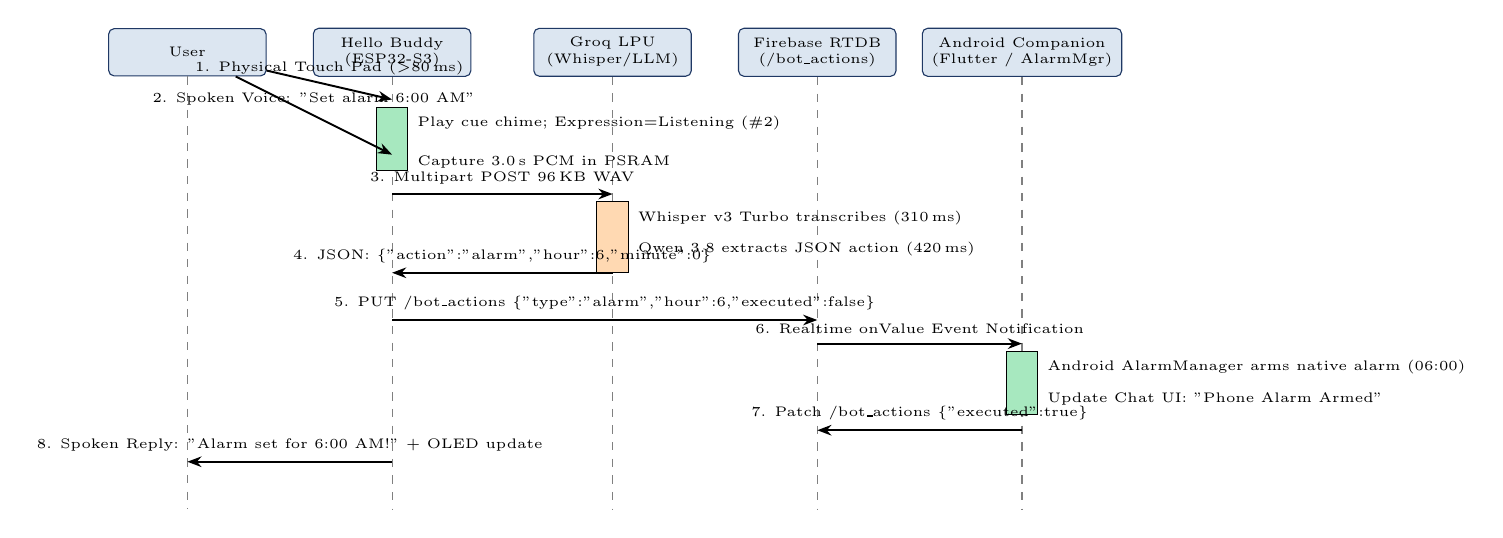
\begin{tikzpicture}[font=\tiny,
 entity/.style={draw=NavyBlue,fill=LightBlue,rounded corners=2pt,align=center,minimum width=2.0cm,minimum height=0.6cm},
 msg/.style={-{Stealth[length=1.8mm]},line width=0.7pt}]

 % Lifeline headers
 \node[entity] (usr) at (0,0) {User};
 \node[entity] (bot) at (2.6,0) {Hello Buddy\\(ESP32-S3)};
 \node[entity] (groq) at (5.4,0) {Groq LPU\\(Whisper/LLM)};
 \node[entity] (fb) at (8.0,0) {Firebase RTDB\\(/bot\_actions)};
 \node[entity] (app) at (10.6,0) {Android Companion\\(Flutter / AlarmMgr)};

 % Vertical Lifelines
 \draw[dashed,black!50] (usr)--(0,-5.8);
 \draw[dashed,black!50] (bot)--(2.6,-5.8);
 \draw[dashed,black!50] (groq)--(5.4,-5.8);
 \draw[dashed,black!50] (fb)--(8.0,-5.8);
 \draw[dashed,black!50] (app)--(10.6,-5.8);

 % Interactions
 \draw[msg] (usr)--(2.6,-0.6) node[midway,above] {1. Physical Touch Pad ($>$80\,ms)};
 \draw[fill=BuddyGreen!40] (2.4,-0.7) rectangle (2.8,-1.5);
 \node[right,font=\tiny] at (2.8,-0.9) {Play cue chime; Expression=Listening (\#2)};
 \draw[msg] (usr)--(2.6,-1.3) node[midway,above] {2. Spoken Voice: ''Set alarm 6:00 AM''};
 \node[right,font=\tiny] at (2.8,-1.4) {Capture 3.0\,s PCM in PSRAM};

 \draw[msg] (2.6,-1.8)--(5.4,-1.8) node[midway,above] {3. Multipart POST 96\,KB WAV};
 \draw[fill=orange!30] (5.2,-1.9) rectangle (5.6,-2.8);
 \node[right,font=\tiny] at (5.6,-2.1) {Whisper v3 Turbo transcribes (310\,ms)};
 \node[right,font=\tiny] at (5.6,-2.5) {Qwen 3.8 extracts JSON action (420\,ms)};
 \draw[msg] (5.4,-2.8)--(2.6,-2.8) node[midway,above] {4. JSON: \{"action":"alarm","hour":6,"minute":0\}};

 \draw[msg] (2.6,-3.4)--(8.0,-3.4) node[midway,above] {5. PUT /bot\_actions \{"type":"alarm","hour":6,"executed":false\}};
 \draw[msg] (8.0,-3.7)--(10.6,-3.7) node[midway,above] {6. Realtime onValue Event Notification};
 \draw[fill=BuddyGreen!40] (10.4,-3.8) rectangle (10.8,-4.6);
 \node[right,font=\tiny] at (10.8,-4.0) {Android AlarmManager arms native alarm (06:00)};
 \node[right,font=\tiny] at (10.8,-4.4) {Update Chat UI: ''Phone Alarm Armed''};
 \draw[msg] (10.6,-4.8)--(8.0,-4.8) node[midway,above] {7. Patch /bot\_actions \{"executed":true\}};

 \draw[msg] (2.6,-5.2)--(0,-5.2) node[midway,above] {8. Spoken Reply: ''Alarm set for 6:00 AM!'' + OLED update};
\end{tikzpicture}
\caption{End-to-end voice-to-alarm execution sequence across embedded, cloud, and mobile layers}\label{fig:interaction_seq}
\end{figure}

\section{Technical Specifications}\label{sec:specs}
\index{specifications}

\begin{table}[H]\centering\small
\caption{Comprehensive technical specifications}
\begin{tabularx}{\linewidth}{|l|X|}\hline
\hdr{Parameter} & \hdr{Design Specification / Value}\\ \hline
Product Model & \ProductName\ (\ModelNo) \\ \hline
Main Controller & Espressif ESP32-S3-WROOM-1 (Dual-Core 32-bit Xtensa LX7 @ 240\,MHz) \\ \hline
Memory & 16\,MB SPI Quad-Flash; 8\,MB Octal PSRAM (OPI Mode enabled) \\ \hline
Visual Display & 1.3-inch SH1106 128$\times$64 White OLED (4-Wire Software SPI) \\ \hline
Microphone & INMP441 Omnidirectional Digital MEMS; 24-bit I2S; SNR 61\,dB \\ \hline
Audio Amplifier & MAX98357A I2S Class-D DAC/Amp (3.2\,W into 4\,$\Omega$ at 5\,V, THD+N 0.05\%) \\ \hline
Speaker & 3\,W, 4\,$\Omega$, 40\,mm diameter dynamic speaker in tuned acoustic chamber \\ \hline
Touch Input & TTP223 Capacitive Touch sensor with hardware rising-edge filter \\ \hline
Wireless Interface & 2.4\,GHz Wi-Fi (802.11 b/g/n, WPA2-PSK); Bluetooth 5.0 LE \\ \hline
Power Supply & 5.0\,V\,DC $\pm$5\% via USB Type-C connector \\ \hline
Current Consumption & Standby / Idle: 110\,mA; Listening: 140\,mA; Speaking (Peak): 420\,mA \\ \hline
Operating Temperature & 0\,\textdegree C to 40\,\textdegree C; 10\% to 85\% RH (non-condensing) \\ \hline
Physical Dimensions & 110\,mm (Height) $\times$ 95\,mm (Width) $\times$ 85\,mm (Depth) \\ \hline
Net Weight & 235\,g $\pm$10\,g (including 3D PLA chassis and components) \\ \hline
Firmware Version & Unified Firmware v\FWVer\ (Native dual-slot I2S, Groq STT/LLM) \\ \hline
\end{tabularx}
\end{table}

% =====================================================================
%  CHAPTER 3: INSTALLATION AND SETUP
% =====================================================================
\chapter{Installation and Setup}\label{ch:install}
\index{installation}\index{setup}

\section{Site Selection and Acoustic Guidelines}
To achieve optimal voice recognition and clear audio playback:
\begin{itemize}[leftmargin=*]
\item Place \ProductName\ on a solid, vibration-free desk surface within comfortable reaching distance (0.3--0.8\,m).
\item Maintain at least 5\,cm clearance behind the robot to allow the speaker sound wave to reflect naturally without acoustic muffling.
\item Do not place the robot next to continuous noise sources such as open computer fans, room air conditioners, or loud desktop speakers.
\item Ensure reliable 2.4\,GHz Wi-Fi coverage at the desk location.
\end{itemize}

\section{Connecting Power}
\begin{warning}
Use only certified 5\,V USB power adapters providing at least 1.5\,A (2.0\,A recommended). Never power the robot from unverified 9\,V/12\,V QuickCharge adapters that do not safely negotiate 5\,V default output.
\end{warning}

\begin{enumerate}[leftmargin=*]
\item Connect the supplied USB-C braided cable to the port on the lower rear of \ProductName\ \callout{5}.
\item Connect the opposite USB-A end to the 5\,V/2\,A wall adapter and insert the adapter into a mains wall outlet.
\item The OLED screen immediately initializes, displaying the boot face and the status text \ui{Booting...}.
\item Within 400\,ms, the robot plays a hardware self-test chime through the speaker, verifying both the I2S DAC and PSRAM audio buffers.
\end{enumerate}

\section{Network Connection and Provisioning}
\ProductName\ requires an active 2.4\,GHz Wi-Fi connection with Internet access to communicate with cloud AI models and Firebase:
\begin{enumerate}[leftmargin=*]
\item The device connects automatically to the configured Wi-Fi credentials (\ui{WIFI\_SSID}). The display shows \ui{WiFi...} with rolling progress dots.
\item Upon successful association, the screen transitions to the neutral face and displays the assigned local IP address (e.g., \ui{IP: 192.168.1.45}) for 800\,ms.
\item The robot announces: \emph{''Hello! I am your buddy. Touch me to talk!''}.
\item \ProductName\ is now in its active idle state (\ui{Ready :)}).
\end{enumerate}

\begin{tip}
If Wi-Fi fails to connect within 15 seconds, the robot displays the alert face and status \ui{No WiFi}. Verify your router's 2.4\,GHz band is active (5\,GHz-only networks are not supported by the 2.4\,GHz radio).
\end{tip}

\section{Companion Mobile App Setup}
The Flutter companion app provides real-time dashboard telemetry, music streaming, and bidirectional action synchronization:
\begin{enumerate}[leftmargin=*]
\item Install \textbf{Hello Buddy Companion} on your Android smartphone (Android 10.0 or later).
\item Launch the application. The app connects to the shared Firebase Realtime Database path:
\begin{center}\texttt{https://epd2026-127ec-default-rtdb.firebaseio.com/users/default}\end{center}
\item On the \menu{Cockpit} tab, observe the status badge in the top right. It will turn solid lime green with the label \ui{ONLINE} and display the robot's local IP address and expression state in real-time.
\end{enumerate}

% =====================================================================
%  CHAPTER 4: OPERATION
% =====================================================================
\chapter{Operation}\label{ch:operation}
\index{operation}

\section{Power States and Modes}
\begin{table}[H]\centering\small
\caption{System operating state matrix}
\begin{tabularx}{\linewidth}{|l|c|l|X|}\hline
\hdr{State} & \hdr{Expression} & \hdr{Label} & \hdr{Hardware Activity}\\ \hline
Idle / Ready & Neutral / Happy & Current task & OLED animated blinking; periodic telemetry (30\,s)\\ \hline
Listening & Focused (\#2) & \ui{LISTENING...} & INMP441 I2S DMA stereo recording (3.0 seconds)\\ \hline
Thinking & Pleased (\#5) & \ui{THINKING...} & Groq Whisper STT + LLM prompt inference\\ \hline
Speaking & Neutral (\#0) & \ui{SPEAKING...} & MAX98357A I2S audio playback from PSRAM\\ \hline
Pomodoro & Focused (\#2) & Time remaining & Active countdown ticker; overdue alert triggers\\ \hline
Quiet / Error & Sleepy (\#7) & \ui{TOO QUIET} & Audio below 20 amplitude; prompts user to repeat\\ \hline
\end{tabularx}
\end{table}

\section{Animated Emotional Expressions}
\ProductName\ communicates mood through procedural OLED eye animations rendered at 25 frames per second:
\begin{figure}[H]\centering
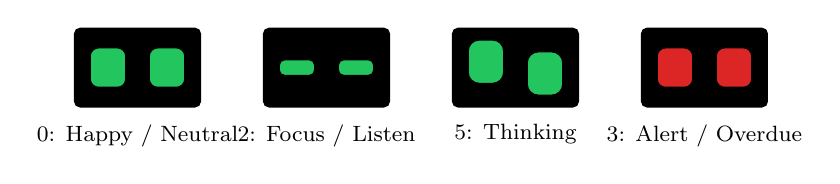
\begin{tikzpicture}[font=\footnotesize]
 % Expression 0: Happy / Neutral
 \draw[fill=black,rounded corners=2pt] (0,0) rectangle (1.6,1.0);
 \draw[fill=BuddyGreen,rounded corners=3pt] (0.2,0.25) rectangle (0.65,0.75);
 \draw[fill=BuddyGreen,rounded corners=3pt] (0.95,0.25) rectangle (1.4,0.75);
 \node[below] at (0.8,-0.1) {0: Happy / Neutral};

 % Expression 2: Focus / Listening
 \draw[fill=black,rounded corners=2pt] (2.4,0) rectangle (4.0,1.0);
 \draw[fill=BuddyGreen,rounded corners=2pt] (2.6,0.4) rectangle (3.05,0.6);
 \draw[fill=BuddyGreen,rounded corners=2pt] (3.35,0.4) rectangle (3.8,0.6);
 \node[below] at (3.2,-0.1) {2: Focus / Listen};

 % Expression 5: Thinking
 \draw[fill=black,rounded corners=2pt] (4.8,0) rectangle (6.4,1.0);
 \draw[fill=BuddyGreen,rounded corners=4pt] (5.0,0.3) rectangle (5.45,0.85);
 \draw[fill=BuddyGreen,rounded corners=4pt] (5.75,0.15) rectangle (6.2,0.7);
 \node[below] at (5.6,-0.1) {5: Thinking};

 % Expression 3: Alert
 \draw[fill=black,rounded corners=2pt] (7.2,0) rectangle (8.8,1.0);
 \draw[fill=AlertRed,rounded corners=3pt] (7.4,0.25) rectangle (7.85,0.75);
 \draw[fill=AlertRed,rounded corners=3pt] (8.15,0.25) rectangle (8.6,0.75);
 \node[below] at (8.0,-0.1) {3: Alert / Overdue};
\end{tikzpicture}
\caption{Representative OLED emotional eye expressions}\label{fig:expressions}
\end{figure}

\section{Voice Interaction Workflow}\label{sec:voice}
Voice commands allow full hands-free control of \ProductName:
\begin{enumerate}[leftmargin=*]
\item \textbf{Initiate Interaction:} 
  \begin{itemize}
  \item \emph{Method A (Touch):} Firmly touch the crown touch sensor \callout{2}.
  \item \emph{Method B (App):} Tap \ui{[🎤 Mic Listen]} on the mobile Cockpit screen.
  \item \emph{Method C (Serial):} Send \texttt{talk} in the Arduino Serial Monitor.
  \end{itemize}
\item \textbf{Acoustic Cue:} The robot plays a chime tone and displays \ui{LISTENING...}.
\item \textbf{Speak Your Command:} Speak naturally toward the front microphone within the 3.0-second recording window (e.g., \emph{''What is the weather today?''}, \emph{''Set an alarm for 7:00 AM''}, or \emph{''Start a 25 minute pomodoro''}).
\item \textbf{Processing:} The robot displays \ui{THINKING...}. Audio is processed through Groq Whisper Large-v3-Turbo and the LLM inference engine.
\item \textbf{Response and Action:} The robot displays the recognized text, speaks the spoken reply through its speaker, and simultaneously executes any parsed actions.
\end{enumerate}

\section{Natural Language Action Dispatch (Alarms, Calendar, Tasks)}
When you speak an action request, \ProductName's LLM engine parses your sentence into a structured JSON dispatch that writes directly to Firebase:
\begin{itemize}[leftmargin=*]
\item \textbf{Alarm Command:} \emph{''Wake me up at 6:30 AM tomorrow morning.''}
\begin{itemize}
\item Robot Reply: \emph{''Alarm set for 6:30 AM.''}
\item Action Payload pushed to \texttt{/users/default/bot\_actions}:
\begin{center}\texttt{\{"type":"alarm", "title":"Wake Up", "hour":6, "minute":30, "executed":false\}}\end{center}
\item The Android companion app's background listener receives this payload and immediately schedules the phone's native \texttt{AlarmManager}.
\end{itemize}
\item \textbf{Calendar Event:} \emph{''Schedule product review on Thursday at 3 PM.''}
\begin{itemize}
\item Dispatched to Android Calendar Provider; inserted into your device calendar.
\end{itemize}
\item \textbf{Task Creation:} \emph{''Add task submit EPD documentation.''}
\begin{itemize}
\item Pushed to Firebase \texttt{/users/default/tasks} and displayed on the OLED screen.
\end{itemize}
\end{itemize}

\section{Pomodoro Study Loop}
\ProductName\ serves as a physical desktop sentinel to keep your study sessions structured:
\begin{enumerate}[leftmargin=*]
\item Trigger Pomodoro by voice (\emph{''Start Pomodoro''}) or tap \ui{[Start]} on the mobile app.
\item The robot switches to the focused expression (\#2) and initiates a 25-minute study countdown.
\item During the session, the OLED status bar tracks elapsed time.
\item When the 25 minutes expire, \ProductName\ sounds an alert chime and speaks: \emph{''Pomodoro done! Take a break.''}.
\item Tap \ui{[+5m Break]} in the companion app to begin your rest interval.
\end{enumerate}

\section{Companion App Features and User Interface}\label{sec:app_ui}
Figure~\ref{fig:app_screens} illustrates the two primary interfaces of the \ProductName\ Companion Android Application: the \textbf{Sentinel Cockpit Dashboard} (left) and the \textbf{Study \& Scheduling Chat Console} (right).

\begin{figure}[H]\centering
\begin{minipage}{0.48\linewidth}
  \centering
  \IfFileExists{figures/app_cockpit_full.jpg}{%
    \includegraphics[width=\linewidth,height=10.2cm,keepaspectratio]{figures/app_cockpit_full.jpg}%
  }{%
    \IfFileExists{figures/app_cockpit.jpg}{%
      \includegraphics[width=\linewidth,height=10.2cm,keepaspectratio]{figures/app_cockpit.jpg}%
    }{%
      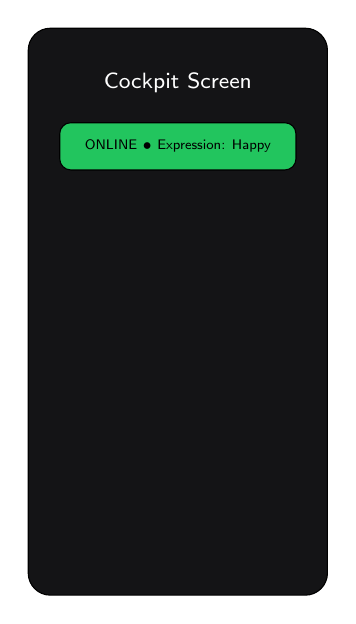
\begin{tikzpicture}
        \draw[fill=BuddyDark,rounded corners=8pt] (0,0) rectangle (3.8,7.2);
        \node[white,font=\sffamily\footnotesize] at (1.9,6.5) {Cockpit Screen};
        \draw[fill=BuddyGreen,rounded corners=4pt] (0.4,5.4) rectangle (3.4,6.0);
        \node[font=\sffamily\tiny] at (1.9,5.7) {ONLINE $\bullet$ Expression: Happy};
      \end{tikzpicture}
    }
  }
  \caption*{1. Sentinel Cockpit Dashboard}\label{fig:cockpit_full_shot}
\end{minipage}\hfill
\begin{minipage}{0.48\linewidth}
  \centering
  \IfFileExists{figures/app_chat_schedule.jpg}{%
    \includegraphics[width=\linewidth,height=10.2cm,keepaspectratio]{figures/app_chat_schedule.jpg}%
  }{%
    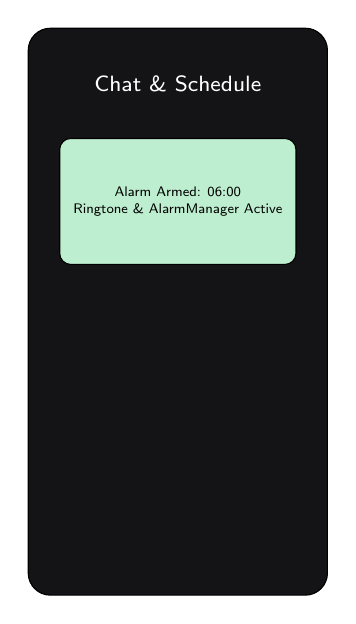
\begin{tikzpicture}
      \draw[fill=BuddyDark,rounded corners=8pt] (0,0) rectangle (3.8,7.2);
      \node[white,font=\sffamily\footnotesize] at (1.9,6.5) {Chat \& Schedule};
      \draw[fill=BuddyGreen!30,rounded corners=4pt] (0.4,4.2) rectangle (3.4,5.8);
      \node[font=\sffamily\tiny,align=center] at (1.9,5.0) {Alarm Armed: 06:00\\Ringtone \& AlarmManager Active};
    \end{tikzpicture}
  }
  \caption*{2. Study \& Scheduling Chat Console}\label{fig:chat_schedule_shot}
\end{minipage}
\caption{Hello Buddy companion Android application core interfaces}\label{fig:app_screens}
\end{figure}

\subsection{Screen 1: Sentinel Cockpit Dashboard}
The Cockpit screen (Figure~\ref{fig:app_screens}, left) provides comprehensive real-time monitoring and immediate tactile control over \ProductName:
\begin{itemize}[leftmargin=*]
\item \textbf{Status Header:} Displays connection state (\ui{ONLINE} in lime green), live device IP address (e.g., \ui{IP: 10.31.177.1...}), current robot expression (\ui{Face: Happy}), and operational uptime.
\item \textbf{Robot Expression \& Audio Deck:} Six one-tap control capsules:
  \begin{itemize}
  \item \ui{[🎯 Focus]}, \ui{[😊 Happy]}, \ui{[💤 Sleep]}, \ui{[😠 Alert]}: Instantly updates the SH1106 OLED procedural eye animation via local REST API and Firebase RTDB.
  \item \ui{[🎤 Mic Listen]}: Remotely triggers the robot's onboard INMP441 microphone recording loop without needing physical contact.
  \item \ui{[🔔 Chime]} and \ui{[🗣️ Speak Text]}: Tests the acoustic speaker and broadcasts arbitrary speech synthesis.
  \end{itemize}
\item \textbf{Weekly Schedule \& Task Checklist:} Calendar date selector bar showing active week days, task counts, and individual task items with quick-action \ui{[MARK DONE]} buttons and category tags (\ui{🤖 AI}, \ui{📅 CAL}).
\item \textbf{Integrated Pomodoro Focus Timer:} Digital 25:00 countdown clock synchronized with the physical robot, featuring \ui{[▶ Start]} and \ui{[+5m Break]} controls.
\end{itemize}

\subsection{Screen 2: Study \& Scheduling Chat Console}
The Chat interface (Figure~\ref{fig:app_screens}, right) provides intelligent conversational scheduling and visual verification of dispatched robot actions:
\begin{itemize}[leftmargin=*]
\item \textbf{Header Controls:} Live RTDB status banner and one-tap \ui{[🎤 Robot Mic]} trigger.
\item \textbf{Subject Context Selector:} Allows setting study context (e.g., \emph{General Engineering \& History}) for tailored conversational assistance.
\item \textbf{Action Execution Card:} When an alarm command is spoken (e.g., \emph{''Set alarm for 6:00 AM tomorrow morning''}), Buddy confirms the schedule and renders a structured green dispatch card:
  \begin{itemize}
  \item \textbf{Phone Alarm Confirmation:} Verifies native Android \texttt{AlarmManager} registration and ringtone arming for 06:00.
  \item \textbf{Robot Sync Badge:} Confirms the alarm was written to Firebase RTDB and synchronized to the robot's OLED display.
  \item \textbf{Action Buttons:} Interactive \ui{[🔔 Test Ringtone]} and \ui{[⏹ Silence]} buttons to preview and silence the alarm.
  \item \textbf{OLED Push Capsule:} \ui{[📺 Push ''Alarm set!'' to OLED]} sends immediate graphical confirmation text to the robot's physical display.
  \end{itemize}
\item \textbf{Multimodal Quick Actions:} Bottom capsules for \ui{[📅 Voice Schedule]}, \ui{[📷 Scan Note/Formula]} (vision input), and visual flow diagrams.
\end{itemize}

% =====================================================================
%  CHAPTER 5: MAINTENANCE
% =====================================================================
\chapter{Maintenance}\label{ch:maint}
\index{maintenance}

\section{Preventive Maintenance Schedule}
\begin{table}[H]\centering\small
\caption{Periodic maintenance inspection schedule}
\begin{tabularx}{\linewidth}{|l|X|l|}\hline
\hdr{Interval} & \hdr{Maintenance Action} & \hdr{Personnel}\\ \hline
Daily / Before Use & Inspect USB-C cable for insulation wear or loose connector fit & User \\ \hline
Monthly & Clean the OLED screen and clear dust from acoustic openings & User \\ \hline
Bi-Annually & Inspect firmware version and flash updates from repository & User / Tech \\ \hline
Annually & Acoustic check: Run self-test tone to verify speaker coil integrity & Technician \\ \hline
\end{tabularx}
\end{table}

\section{Cleaning Instructions}\label{sec:cleaning}
\begin{enumerate}[leftmargin=*]
\item Disconnect the USB-C power cable from the rear of the robot before cleaning.
\item Gently wipe the SH1106 OLED display using a dry, soft optical microfiber cloth.
\item Clean the 3D-printed PLA housing using a clean cloth lightly dampened with pure water. Dry thoroughly with a microfiber towel.
\item Use a dry, soft-bristled brush or low-pressure dry air canister to remove accumulated dust from the microphone aperture \callout{3} and rear speaker grille \callout{4}.
\end{enumerate}

\begin{notice}
Never use isopropyl alcohol, acetone, benzene, window cleaner, or abrasive scouring pads on the acrylic OLED window or PLA housing. Solvents will craze and cloud the display.
\end{notice}

\section{Firmware Updating}\label{sec:fw}
To update \ProductName\ to the latest firmware release:
\begin{enumerate}[leftmargin=*]
\item Download the updated \texttt{hello\_buddy.ino} from the official project repository.
\item Connect \ProductName\ to your computer using the USB-C data cable.
\item Open the sketch in **Arduino IDE 2.x**. Ensure board settings:
  \begin{itemize}
  \item Board: \ui{ESP32S3 Dev Module}
  \item PSRAM: \ui{OPI PSRAM} (Mandatory for audio buffers)
  \item Flash Size: \ui{16MB (128Mb)}
  \end{itemize}
\item Click \ui{Upload}. Do not disconnect the USB cable until the IDE reports \ui{Leaving... Hard resetting via RTS pin...}.
\end{enumerate}

% =====================================================================
%  CHAPTER 6: TROUBLESHOOTING
% =====================================================================
\chapter{Troubleshooting}\label{ch:trouble}
\index{troubleshooting}

\section{Diagnostic Decision Tree}
\begin{figure}[H]\centering
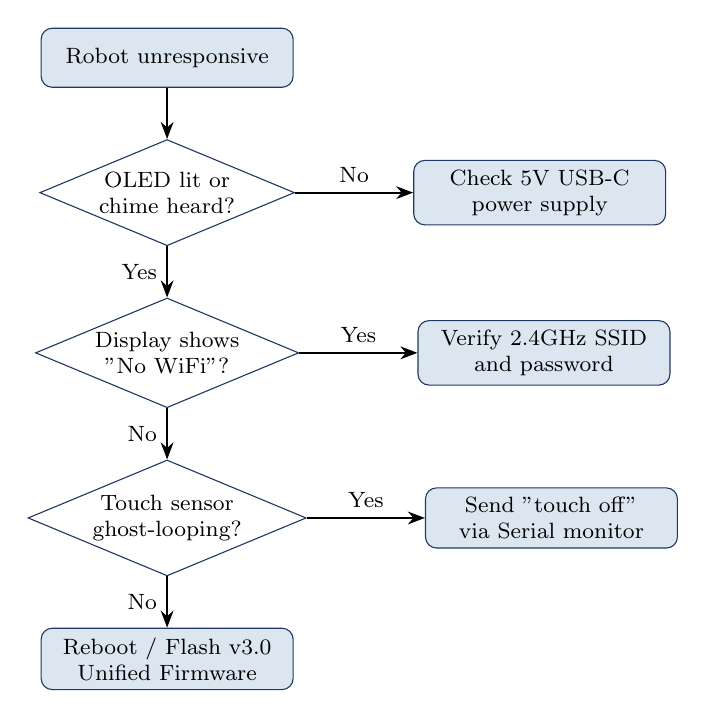
\begin{tikzpicture}[node distance=0.65cm,font=\footnotesize,
 st/.style={draw=NavyBlue,fill=LightBlue,rounded corners=4pt,minimum width=3.2cm,minimum height=0.75cm,align=center},
 dc/.style={draw=NavyBlue,fill=white,diamond,aspect=2.4,inner sep=1pt,align=center},
 ar/.style={-{Stealth},line width=0.7pt}]

 \node[st] (start) {Robot unresponsive};
 \node[dc,below=of start] (d1) {OLED lit or\\chime heard?};
 \node[st,right=1.5cm of d1] (s1) {Check 5V USB-C\\power supply};
 \node[dc,below=of d1] (d2) {Display shows\\''No WiFi''?};
 \node[st,right=1.5cm of d2] (s2) {Verify 2.4GHz SSID\\and password};
 \node[dc,below=of d2] (d3) {Touch sensor\\ghost-looping?};
 \node[st,right=1.5cm of d3] (s3) {Send ''touch off''\\via Serial monitor};
 \node[st,below=of d3] (s4) {Reboot / Flash v\FWVer\\Unified Firmware};

 \draw[ar] (start)--(d1);
 \draw[ar] (d1)--node[above]{No}(s1);
 \draw[ar] (d1)--node[left]{Yes}(d2);
 \draw[ar] (d2)--node[above]{Yes}(s2);
 \draw[ar] (d2)--node[left]{No}(d3);
 \draw[ar] (d3)--node[above]{Yes}(s3);
 \draw[ar] (d3)--node[left]{No}(s4);
\end{tikzpicture}
\caption{System diagnostic flow diagram}\label{fig:diag}
\end{figure}

\section{Symptoms, Causes, and Solutions}
\begin{table}[H]\centering\small
\caption{Detailed fault resolution table}
\begin{tabularx}{\linewidth}{|p{0.25\linewidth}|X|X|}\hline
\hdr{Observed Symptom} & \hdr{Probable Root Cause} & \hdr{Recommended Solution}\\ \hline
Robot continuously enters listening mode without touch & Sensor pin floated or inverted active level triggered & Fixed in v\FWVer\ with rising-edge debounce. Send \texttt{touch off} via Serial to disable pin if hardware is disconnected.\\ \hline
OLED shows \ui{NOT HEARD} or Wit.ai returns \ui{0} & Low microphone volume, upload timeout, or network latency & Speak clearly within 0.5\,m. Dual-pipeline now routes primary audio to Groq Whisper STT (300\,ms).\\ \hline
Display stuck on \ui{PSRAM ERROR} & Octal PSRAM not enabled in compiler settings & In Arduino IDE, select \menu{Tools $\rightarrow$ PSRAM $\rightarrow$ OPI PSRAM} and re-upload firmware.\\ \hline
Companion app shows yellow-black hazard stripes & Mobile screen width overflow on older APK build & Fixed in current Dart build. Run \texttt{build\_apk.ps1} and reinstall the latest \texttt{app-debug.apk} on your phone.\\ \hline
Spoken alarms not ringing on Android phone & Bot actions not marked executed or app permissions missing & Ensure Hello Buddy Companion has permission for Alarms and Reminders under Android system settings.\\ \hline
Audio distorted or clipping during speech & MAX98357A gain too high or supply voltage dropping below 4.7\,V & Use a high-quality 5\,V/2\,A power adapter and thick-gauge USB-C cable.\\ \hline
\end{tabularx}
\end{table}

\section{Firmware Error Codes}\index{error codes}
\begin{table}[H]\centering\small
\caption{Firmware status and diagnostic error codes}
\begin{tabularx}{\linewidth}{|c|l|X|}\hline
\hdr{Code} & \hdr{Display Message} & \hdr{Corrective Action}\\ \hline
E01 & \ui{No WiFi} & Router unreachable; verify 2.4\,GHz credentials in \texttt{hello\_buddy.ino}\\ \hline
E02 & \ui{PSRAM ERROR} & Memory allocation failed; verify ESP32-S3 N16R8 board selection\\ \hline
E03 & \ui{TOO QUIET} & Microphone captured amplitude $<$20; speak closer to microphone\\ \hline
E04 & \ui{NOT HEARD} & Both Groq Whisper and Wit.ai failed to parse transcript; re-trigger voice\\ \hline
E05 & \ui{Groq 404} & Model deprecated; verify active model ID (\texttt{qwen/qwen3.8-27b})\\ \hline
E06 & \ui{Firebase -1} & TLS socket dropped; check Internet gateway and restart robot\\ \hline
\end{tabularx}
\end{table}

% =====================================================================
%  CHAPTER 7: DISPOSAL AND ENVIRONMENT
% =====================================================================
\chapter{Disposal and Environment}\label{ch:disposal}
\index{disposal}\index{recycling}

\section{WEEE Directive and E-Waste Compliance}
\begin{center}\weeesym[1.1cm]\end{center}
The crossed-out wheeled bin symbol indicates that \ProductName\ must not be disposed of with ordinary household waste. In compliance with the \textbf{E-Waste (Management) Rules, India} and the European \textbf{WEEE Directive 2012/19/EU}, electronic products must be collected separately for environmentally sound recycling and material recovery.

\section{Decommissioning Procedure}
Prior to submitting the product for recycling:
\begin{enumerate}[leftmargin=*]
\item \textbf{Data Wipe:} In the companion mobile app, delete task records and clear voice logs stored under your Firebase database path.
\item \textbf{Power Disconnect:} Disconnect and separate the external USB-C power supply adapter.
\item \textbf{Authorized Handover:} Deposit the unit at an authorized institutional or municipal electronic waste collection center.
\end{enumerate}

\section{Material Composition Breakdown}
\begin{table}[H]\centering\small
\caption{Material composition for recyclers}
\begin{tabularx}{\linewidth}{|l|X|l|}\hline
\hdr{Component} & \hdr{Dominant Material} & \hdr{Recycling Stream}\\ \hline
Main Enclosure & Polylactic Acid (PLA) 3D-printed thermoplastic & Industrial compost / Plastics \\ \hline
Electronics & FR-4 laminate, copper traces, lead-free SAC305 solder & Precious metal e-waste recovery \\ \hline
Display Window & PMMA Acrylic / OLED Glass & Specialized glass recycling \\ \hline
Packaging & Unbleached corrugated cardboard & Standard paper/cardboard stream \\ \hline
\end{tabularx}
\end{table}

% =====================================================================
%  CHAPTER 8: WARRANTY, SUPPORT, AND COMPLIANCE
% =====================================================================
\chapter{Warranty, Support and Compliance}\label{ch:compliance}

\section{Academic Prototype Warranty}
\ProductName\ is warranted for a period of \textbf{12 months} from the date of lab evaluation against defects in firmware functionality and component assembly when operated under designated parameters.

\textbf{Warranty Exclusions:} Damage resulting from over-voltage power supplies ($>$5.5\,V), liquid ingress, unauthorized mechanical modification, or thermal exposure beyond 50\,\textdegree C.

\section{Technical Support Contacts}
\begin{table}[H]\centering\small
\caption{Support and institutional contact details}
\begin{tabular}{|l|l|}\hline
\hdr{Channel} & \hdr{Contact Information}\\ \hline
Project Email & \SupportMail \\ \hline
Developer Lead & Ziaur Rahaman (Roll No.\ 2404154), Group 09 \\ \hline
Institution & School of Electronics Engineering, KIIT Deemed to be University \\ \hline
Lab Facility & Electronic Product Development (Sessional) Laboratory \\ \hline
Code Repository & \url{https://github.com/ziaur-rahaman/hello-buddy} \\ \hline
\end{tabular}
\end{table}

\section{Regulatory Pre-Compliance Matrix}
\begin{table}[H]\centering\small
\caption{Standard pre-compliance evaluation}
\begin{tabularx}{\linewidth}{|l|l|l|}\hline
\hdr{Evaluation Area} & \hdr{Standard Specification} & \hdr{Status / Conformity}\\ \hline
Electrical Safety & IEC 62368-1:2018 (Audio/video, ICT equipment) & Pre-compliant (SELV 5V DC supply) \\ \hline
EMC Emissions & CISPR 32 / EN 55032 Class B (Residential) & Pre-compliant (Internal ground planes) \\ \hline
Hazardous Substances & RoHS Directive 2011/65/EU & Complies (Lead-free components) \\ \hline
Manual Instructions & IEC/IEEE 82079-1:2019 & Fully Compliant (This document) \\ \hline
\end{tabularx}
\end{table}

% =====================================================================
%  APPENDICES
% =====================================================================
\appendix
\chapter{Quick Reference Cheat Sheet}
\begin{table}[H]\centering\small
\caption{Voice commands and quick operational controls}
\begin{tabularx}{\linewidth}{|l|X|}\hline
\hdr{Desired Goal} & \hdr{Spoken Phrase or Trigger Action}\\ \hline
Ask for Weather & \emph{''What's the weather today in Bhubaneswar?''} \\ \hline
Set Morning Alarm & \emph{''Set an alarm for 6:30 AM tomorrow''} \\ \hline
Start Focus Timer & \emph{''Start a 25 minute pomodoro''} \\ \hline
Add Study Task & \emph{''Add a task to complete my EPD report''} \\ \hline
Check System Uptime & \emph{''How long have you been awake?''} \\ \hline
Physical Touch Trigger & Touch crown capacitive pad for $>$80\,ms \\ \hline
Emergency Hardware Reboot & Hold recessed \ui{[R]} button for 2 seconds \\ \hline
Serial Commands & \texttt{talk}, \texttt{chime}, \texttt{alert}, \texttt{touch on}, \texttt{touch off}, \texttt{say <text>} \\ \hline
\end{tabularx}
\end{table}

\chapter{Hardware Pinout and Schematic Interfaces}
\begin{table}[H]\centering\small
\caption{ESP32-S3 N16R8 physical pin mapping (Technician Only)}
\begin{tabularx}{\linewidth}{|l|c|l|X|}\hline
\hdr{Subsystem} & \hdr{GPIO} & \hdr{Pin Name} & \hdr{Hardware Connection / Notes}\\ \hline
Capacitive Touch & GPIO 3 & \texttt{TOUCH\_PIN} & TTP223 Out (Active-HIGH, 80\,ms edge filter) \\ \hline
OLED Clock & GPIO 4 & \texttt{OLED\_SCK} & SH1106 Serial Clock (4-Wire Software SPI) \\ \hline
OLED Data & GPIO 5 & \texttt{OLED\_SDA} & SH1106 Master Out (MOSI / D1) \\ \hline
OLED Reset & GPIO 6 & \texttt{OLED\_RES} & SH1106 Hardware Reset \\ \hline
OLED Data/Command & GPIO 7 & \texttt{OLED\_DC} & SH1106 Command (Low) / Data (High) selector \\ \hline
OLED Chip Select & GPIO 15 & \texttt{OLED\_CS} & SH1106 Active-Low Slave Select \\ \hline
Speaker Bit Clock & GPIO 39 & \texttt{SPK\_BCLK} & MAX98357A I2S0 Bit Clock \\ \hline
Speaker Word Select & GPIO 38 & \texttt{SPK\_LRC} & MAX98357A I2S0 Left/Right Clock \\ \hline
Speaker Audio Data & GPIO 48 & \texttt{SPK\_DIN} & MAX98357A I2S0 Serial Data In \\ \hline
Microphone Bit Clock & GPIO 42 & \texttt{MIC\_SCK} & INMP441 I2S0 Bit Clock \\ \hline
Microphone Word Select & GPIO 41 & \texttt{MIC\_WS} & INMP441 I2S0 Word Select \\ \hline
Microphone Serial Data & GPIO 40 & \texttt{MIC\_SD} & INMP441 I2S0 Serial Data Out \\ \hline
\end{tabularx}
\end{table}

\chapter{Local REST Web API Specification}
\begin{table}[H]\centering\small
\caption{Onboard HTTP server endpoints (Port 80)}
\begin{tabularx}{\linewidth}{|l|l|l|X|}\hline
\hdr{HTTP Method} & \hdr{URI Endpoint} & \hdr{Request Payload} & \hdr{Response / Behavior}\\ \hline
\texttt{GET} & \texttt{/status} & None & Returns JSON telemetry (IP, uptime, expression, tasks) \\ \hline
\texttt{POST} & \texttt{/listen} & None & Immediately triggers 3.0\,s voice interaction loop \\ \hline
\texttt{POST} & \texttt{/emotion} & \texttt{\{"state": 2\}} & Overrides OLED expression (0--7) \\ \hline
\texttt{POST} & \texttt{/tone} & \texttt{\{"type":"chime"\}} & Plays onboard synthesized acoustic alert tone \\ \hline
\texttt{POST} & \texttt{/pomodoro} & \texttt{\{"action":"start"\}} & Starts or cancels the Pomodoro focus timer \\ \hline
\texttt{POST} & \texttt{/touch} & \texttt{\{"enabled":true\}} & Software toggle for hardware touch sensor pin \\ \hline
\texttt{POST} & \texttt{/speak} & \texttt{\{"text":"Hello"\}} & Synthesizes text via Groq TTS and speaks aloud \\ \hline
\end{tabularx}
\end{table}

\chapter{Glossary of Technical Terms}
\begin{tabular}{lp{0.75\linewidth}}
\textbf{DMA} & Direct Memory Access; streams audio to/from hardware pins without CPU polling.\\
\textbf{Groq LPU} & Language Processing Unit; ultra-low-latency AI tensor inference silicon.\\
\textbf{I2S} & Inter-IC Sound; high-speed serial bus standard for digital audio data.\\
\textbf{MEMS} & Micro-Electro-Mechanical Systems; microscopic silicon sensor microphones.\\
\textbf{OLED} & Organic Light-Emitting Diode; emissive display technology offering deep contrast.\\
\textbf{PSRAM} & Pseudo-Static Random Access Memory; external RAM (8\,MB Octal) for audio buffers.\\
\textbf{RTDB} & Realtime Database; low-latency cloud synchronization service by Google Firebase.\\
\textbf{STT} & Speech-to-Text; transcribing spoken audio waveform into text strings.\\
\textbf{TTS} & Text-to-Speech; synthesized vocal output generated from textual content.\\
\textbf{WEEE} & Waste Electrical and Electronic Equipment Directive.\\
\end{tabular}

\printindex
\end{document}
